\section{Load Balancing in Fog computing}



\label{s3}

\subsection{Fog Computing Task Model}
\label{Fog Computing Task Model}

% We showed that it is possible to obtain fairly high accuracy with simple linear prediction model. 


In section \ref{s2}, we show that vehicles' mobility pattern can be predicted with high accuracy. For a application such as lane change assistance in connected car, we want to have the data ready for a car when it connects with a new fog server. With the ability to predict which server a car is traveling to, we can perform load balancing and process the tasks before the cars arrive at their predicted locations. 

The task model for connected car system in fog computing is composed of cars, local fog servers and a remote cloud server. The local servers are inter-connected and also connected to the cloud server. A simple system can be illustrated using Figure \ref{opt_rep}. In Figure \ref{opt_rep}, there is one cloud server and three local fog servers, A, B and C. Each fog server is connected to the cars that sit in its wireless range, indicated by hexagons with different colors. We treat the workload from each car as one task. Those tasks are passed through the nearest servers, which can either keep the tasks and do the processing or distribute them to other servers that have extra capacities. So in Figure \ref{opt_rep}, 5 tasks are initially passed to server A, 3 tasks are initially passed to server B and, 4 tasks are initially passed to server C, and the cloud server does not get any initial task.


The general graphical representation of the task model is shown in Figure \ref{opt_gen}. The local servers are interconnected, so they can distribute their tasks among themselves or the remote cloud. In other words, all servers can both accept tasks from other servers and offload tasks to other servers. Each server can have different resources and constraints. Table \ref{fogsysvar} shows the variables used in the task model. In Table \ref{fogsysvar}, $k$ is the number of servers in the system. $N_{i}$ is the number of tasks initially passed to server $i$. Figure \ref{opt_rep} shows an example system with $k=4$, $N_{A}=5$, $N_{B}=4$, $N_{C}=3$, and $N_{cloud}=0$. $B_{ij}$ is the link rate between server $i$ and server $j$. $C_{j}$ is the maximum number of tasks server $j$ can handle. $x$ is the number of CPU cycles required to process each task assuming all tasks consume equal amount of bandwidth. $f_{j}$ is the CPU frequency of server $j$. $D$ is the deadline for each task.  $\tau$ is the allowed processing time for each server. The reason $\tau$ is needed is because we are doing load balancing based on mobility prediction which is calculated periodically. Every time the mobility prediction is updated, load balancing should be performed. In other words, we are restricting the time to process tasks to be less than the deadline so the remaining time can be used for running mobility prediction and load balancing. So $D-\tau$ can be seen as the overhead budget reserved for executing mobility prediction and load balancing. Finally, $n_{ij}$ is the optimizing variable to be solved that tells how many tasks should be offloaded from server $i$ to server $j$. 






\begin{figure}[ht!]
\centering
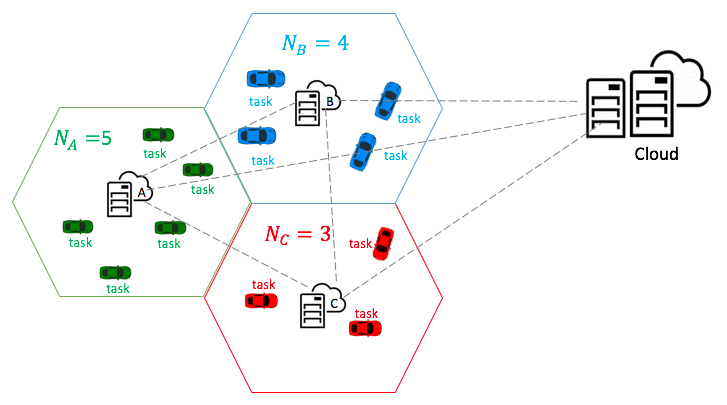
\includegraphics[width=1\linewidth]{images/opt_rep}
\caption{Task Model Example}
\label{opt_rep}
\end{figure}

\begin{figure}[ht!]
\centering
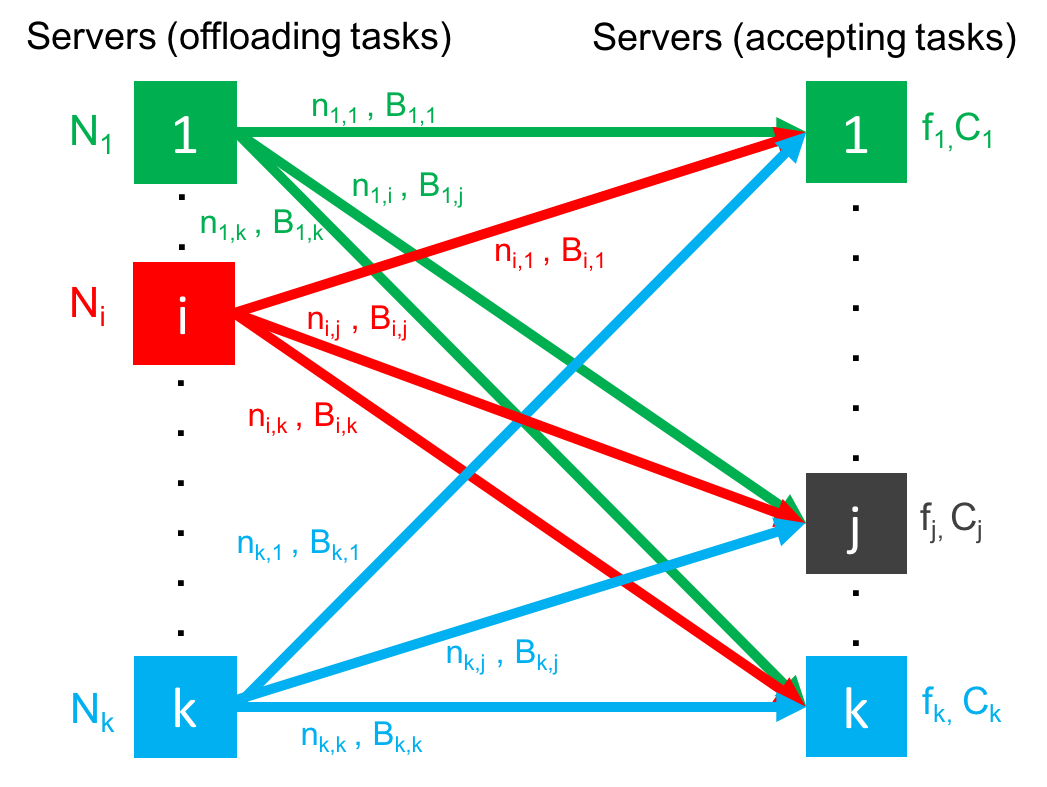
\includegraphics[width=0.8\linewidth]{images/opt_gen}
\caption{Task Model in Fog Computing}
\label{opt_gen}
\end{figure}



\begin{table}[h]
\caption{Parameters \& Variables in the Task Model}
\small
\centering
\begin{tabular}{| m{1cm} |  m{15em} |}
    \hline
    \multicolumn{2}{|l|}{\textbf{Parameters for Servers and Tasks}}\\
    \hline
    $k$ & Number of servers \\
    \hline
    $N_{i}$ & Number of initial tasks for server $i$\\
    \hline
    $B_{ij}$ & Link rate between server $i$ and server $j$ (tasks/sec)\\
    \hline
    $C_{j}$ & Capacity of server $j$ (tasks)\\
    \hline
    $x$ & Number of CPU cycles required for each task (Mcycles)\\
    \hline
    $f_{j}$ & CPU frequency of server $j$ (MHz)\\
    \hline
    $D$ & Deadline for all tasks (sec)\\
    \hline
    $\tau$ & Allowed processing time for each server (sec)\\
    \hline\hline
    \multicolumn{2}{|l|}{\textbf{Optimizing Variables}}\\
    \hline
    $n_{ij}$ & Number of tasks distributed from server $i$ to server $j$\\
    \hline
\end{tabular}
\label{fogsysvar}
\end{table}


 Since we do not know how a server schedules the tasks coming from other servers and the arrival order of those incoming tasks, it is impossible to calculate the completion time for each task that is offloaded to a server. So instead of trying to perform load balancing at the task level, we propose to execute load balancing at the server level by treating the tasks offloaded by other servers as one large aggregated task as illustrated in Figure \ref{opt_agg}. By doing so, we are able to calculate the completion time of the large aggregated task at each server disregarding how that server schedule its tasks and the arrival order of the incoming tasks. 
 


\begin{figure}[ht!]
\centering
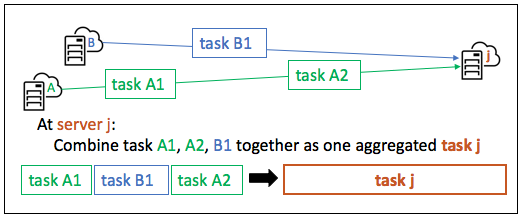
\includegraphics[width=1\linewidth]{images/opt_agg}
\caption{Aggregated Task Example}
\label{opt_agg}
\end{figure}

Now we have defined the concept of an aggregated task at server $j$, we can establish the definitions for the following terms in order to understand the formulation presented next. 
\begin{itemize}[]
\item \textbf{Transmission time for aggregated task at server $j$:} The time for server $i$ to transmit its tasks($n_{ij}$) to server $j$ is $n_{ij}$ divided by the link rate ($B_{ij}$). So the time it takes for all the tasks(aggregated tasks) assigned to server $j$ is the sum of all servers' transmitting time, as shown in (\ref{trans}).
\begin{equation}
\small
\label{trans}
Transmission \ time \ at \ server \ j: \sum\limits_{i=1}^{k} \frac{n_{ij}}{B_{ij}}
\end{equation}


\item \textbf{Turnaround time for aggregated task at server $j$:} The time it takes for server $j$ to process all the tasks offloaded from other servers is calculated by taking the total CPU cycles required, $\sum\limits_{i=1}^{k} n_{ij}*x$, divided by $f_{j}$, the CPU frequency of server $j$, as shown in (\ref{turn}).
\begin{equation}
\small
\label{turn}
Turnaround \ time \ at \ server \ j\ : \sum\limits_{i=1}^{k} \frac{n_{ij}*x}{f_{j}}
\end{equation}

\item
\textbf{Completion time for aggregated task at server $j$:} Completion time at server $j$ is the time it takes to complete its aggregated task. It is the sum of transmission time (\ref{trans}) and turnaroud time (\ref{turn}), as shown in (\ref{comp}).
\begin{equation}
\small
\label{comp}
Completetion \ time \ at \ server \ j\ : \sum\limits_{i=1}^{k} (\frac{n_{ij}}{B_{ij}}+\frac{n_{ij}*x}{f_{j}})
\end{equation}

\item
\textbf{Lateness for aggregated task at server $j$:} Lateness is defined by subtracting completion time (\ref{comp}) with $D$, the deadline, as shown in (\ref{late}).
\begin{equation}
\small
\label{late}
Lateness \ at \ server \ j\ : \left (\sum\limits_{i=1}^{k} (\frac{n_{ij}}{B_{ij}}+\frac{n_{ij}*x}{f_{j}}) \right) - D
\end{equation}

\end{itemize}







\subsection{Problem Formulation}










The objective of the load balancing problem is to minimize deadline misses and total runtime. With the task model in place, we develop a mixed integer program for solving optimal load balancing of tasks across servers. The objective function is shown in (\ref{opt_min}). The optimization goal is to minimize deadline misses and total runtime. To analyze this objective function, first we recognize that $\left (\sum\limits_{i=1}^{k} \frac{n_{ij}}{B_{ij}}+\frac{n_{ij}*x}{f_{j}}\right )-D$ is the lateness of completing aggregated tasks at server $j$, so minimizing this term reflects in minimizing total runtime. Secondly, $v*max\left ( 0, \sum\limits_{i=1}^{k} \frac{n_{ij}}{B_{ij}}+\frac{n_{ij}*x}{f_{j}}\right )$ in (\ref{opt_min}) penalizes tardiness(missed deadlines) of aggregated task at server $j$, so minimizing this term reflects in minimizing deadline misses. Lastly $v$ is used as weighing factor so one can decide to put more emphasis in minimizing deadline misses or total runtime. A more graphical analysis on the objective function (\ref{opt_min}) is shown in Figure \ref{opt_ill}.



\setlength{\arraycolsep}{0.0em}
\small
\begin{eqnarray}
\label{opt_min}
&Min&: \quad \sum_{j=1}^{k}\left [\left (\sum\limits_{i=1}^{k} \frac{n_{ij}}{B_{ij}}+\frac{n_{ij}*x}{f_{j}} \right ) \ - \ D \ + \right.\nonumber\\
&\phantom{min}&\qquad \left.v * max\left ( 0, \sum\limits_{i=1}^{k} \frac{n_{ij}}{B_{ij}}+\frac{n_{ij}*x}{f_{j}}\right )\right ]\\
\label{opt_concpu}
&s.t.& \quad\sum_{i=1}^{k} n_{ij}*x\leq f_{j}*\tau  \qquad for \ j\in \left \{ 1,2,..,k \right \}\\
\label{opt_conc}
&\phantom{s.t.}& \quad\sum_{i=1}^{k} n_{ij}\leq C_{j} \ \ \qquad\quad\quad for \ j\in \left \{ 1,2,..,k \right \}\\
\label{opt_n}
&\phantom{s.t.}& \quad\sum_{j=1}^{k} n_{ij}=N_{i} \  \ \qquad \quad \quad for \ i\in \left \{ 1,2,..,k \right \} \\
\label{opt_int}
&\phantom{s.t.}& \quad n_{ij}\in Z^{+} \qquad \qquad \qquad  for \ i\in \left \{ 1,2,..,k \right \} ,\nonumber\\
&\phantom{s.t.}& \quad\phantom{n_{ij}\in Z^{+}}  \qquad \qquad \qquad for \ j\in \left \{ 1,2,..,k \right \}
\end{eqnarray}
\setlength{\arraycolsep}{5pt}

\begin{figure}[ht!]
\centering
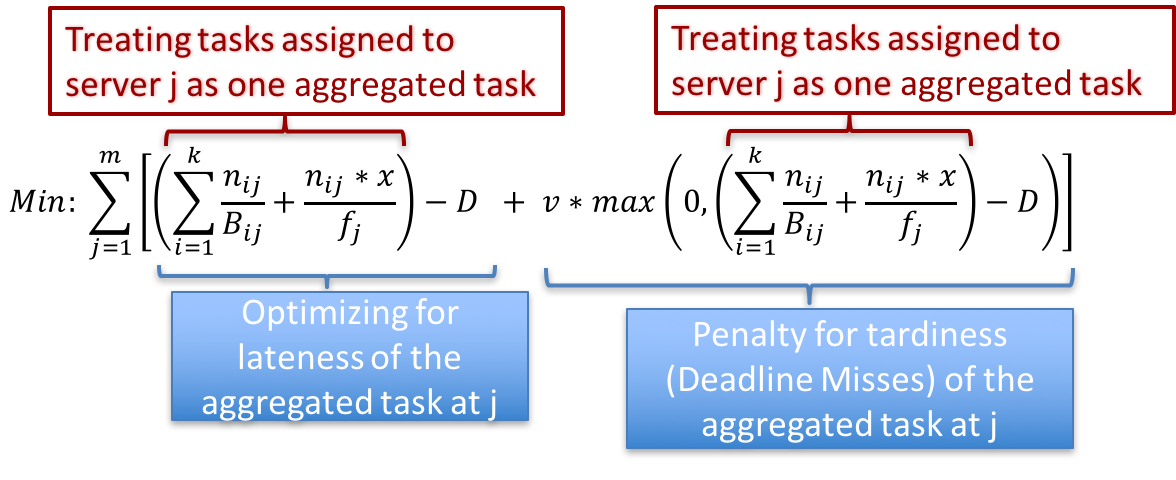
\includegraphics[width=1\linewidth]{images/opt_ill}
\caption{Analysis of Objective Function}
\label{opt_ill}
\end{figure}
\normalsize

The constraints for the optimization are shown from (\ref{opt_concpu}) to (\ref{opt_int}). Constraint (\ref{opt_concpu}) requires that every server has enough CPU cycles available for the tasks offloaded from other servers. Constraint (\ref{opt_conc}) requires the total number of tasks allocated to a server does not exceed its capacity. Constraint (\ref{opt_n}) makes sure that all tasks will be distributed and processed. Constraint (\ref{opt_int}) makes sure a task will not be divided into smaller sub-tasks. Finally we reformulate the objective function (\ref{opt_min}) by introducing $y_{j}$ as shown from (\ref{opt_fstart}) to (\ref{opt_end}) in order to solve the optimization using lp\_solve\cite{lpsolve}.



\setlength{\arraycolsep}{0.0em}
\begin{eqnarray}
\small
\label{opt_fstart}
&Min&: \sum_{j=1}^{k}\left [\left (\sum\limits_{i=1}^{k} \frac{n_{ij}}{B_{ij}}+\frac{n_{ij}*x}{f_{j}} \right ) \ - \ D \ + v * y_{j} \right ]\\
\label{opt_concpu2}
&s.t.& \sum_{i=1}^{k} n_{ij}*x\leq f_{j}*\tau  \qquad for \ j\in \left \{ 1,2,..,k \right \}\\
\label{opt_conc2}
&\phantom{s.t.}& \sum_{i=1}^{k} n_{ij}\leq C_{j} \ \ \qquad\quad\quad for \ j\in \left \{ 1,2,..,k \right \}\\
\label{opt_n2}
&\phantom{s.t.}& \sum_{j=1}^{k} n_{ij}=N_{i} \  \ \qquad \quad \quad for \ i\in \left \{ 1,2,..,k \right \} \\
\label{opt_int2}
&\phantom{s.t.}&  n_{ij}\in Z^{+} \qquad \qquad \qquad  for \ i\in \left \{ 1,2,..,k \right \} ,\nonumber\\
&\phantom{s.t.}& \phantom{n_{ij}\in Z^{+}}  \qquad \qquad \qquad for \ j\in \left \{ 1,2,..,k \right \}\\
\label{opt_y}
&\phantom{s.t.}& y_{j}\geq 0 \ \ \ \qquad\qquad\qquad for \ j\in \left \{ 1,2,..,k \right \}\\
\label{opt_end}
&\phantom{s.t.}& y_{j}\geq \left (\sum\limits_{i=1}^{k} \frac{n_{ij}}{B_{ij}}+\frac{n_{ij}*x}{f_{j}} \right )-D \nonumber\\ 
&\phantom{s.t.}&\qquad\qquad\qquad\qquad\qquad for \ j\in \left \{ 1,2,..,k \right \}
\end{eqnarray}
\setlength{\arraycolsep}{5pt}
\normalsize

